\vspace*{-5mm}
\mysection{Architectural Design}

\mysubsection{Overview}
In this section we describe the architectural arrangement that we designed for EasyLib’s client and server side.\\

The proposed architecture is composed by three tiers:

\begin{itemize}
\item \emph{Presentation Tier:} it’s represented by the tablet and the Mobile Android App;  they constitutes the view part of our system.
\item \emph{Business Tier:} it’s represented by the Socket Server, which responds to the user’s requests, and the Application Server, which contains all the Business Logic. The application server communicates with the DBMS of the MySQL Database contained in the Database Tier.
\item \emph{Database Tier:} it’s represented by the DB Server, that contains and manages persistent data in an efficient way.
\end{itemize}

\vspace*{0cm}
\begin{figure}[H]
	\centering
	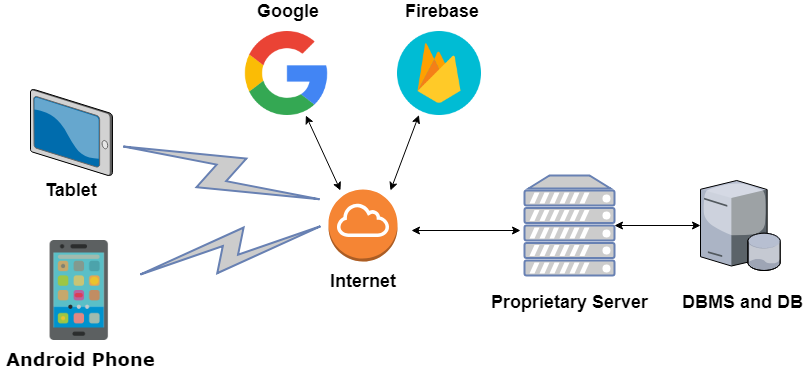
\includegraphics[scale=0.5]{Images/Diagrams/High_level_System_Architecture}
	\caption{High level system architecture}
\end{figure}

\newpage
\mysubsection{High Level Component View}
The system is divided in three main layers: Presentation Layer, Business Layer and Data Layer. The presentation layer is both mobile and tablet application. For both we have a very thin client with the main aim of performing requests to the application server in the Business layer and receives the demanded information to manage and show locally.

\vspace*{0.5cm}
\begin{figure}[H]
	\centering
	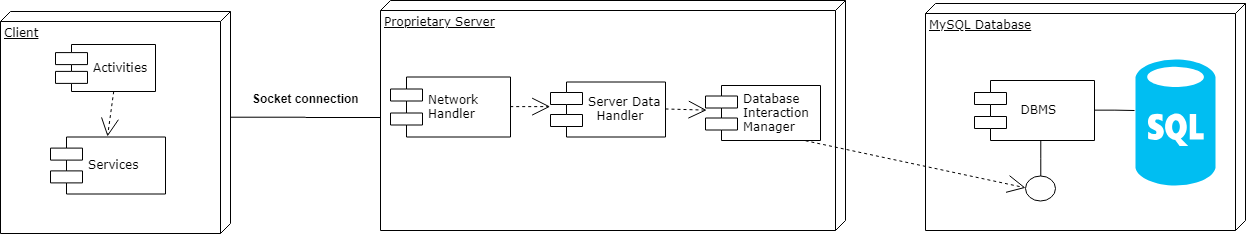
\includegraphics[scale=0.65]{Images/Diagrams/Component_diagram}
	\caption{Component View}
\end{figure}
\vspace*{0cm}
\mysubsubsection{Client-side Application}
In this section we are going to illustrate the general architecture of our client application.EasyLib can be fairly considered in the middle between a thin and a fat client. The data are requested client side and correctly retrieved with the work performed by the application server and the DBMS. Nonetheless, on the client side the data are checked, filtered and formatted in order to give the most pleasant screen view.
\\ 
In order to accomplish efficiently the communication task, the client exploits two different android services: 

\begin{itemize}
\item \emph{Connection service:}it manages the communication with the server. It opens a socket connection and keep it alive in order to send and receive messages in any moment and in an asynchronous fashion.
\item \emph{Check connection service:}It constantly checks if there is internet connection available and if is not the case makes the user aware of this forbidding any dangerous actions that could lead to a misbehaviour of the app.
\end{itemize}

As in the server side, we implemented a system to decode the messages received from the server. Here the task was heavier than the application server homologous due to some Android constraints. In fact the messages have to be passed through two different classes before reaching the application context and be manipulated to modify the view. The service thread is in charge of this massage handling. First of all the message received is used as key in a functional HashMap to trigger the correspondent method that receive the expected object from the input socket channel, wrap it in a bundle and pass it to the next class. Here another functional map allows to call the correct method and send the object along with its related message to current application context where a Broadcast receiver component is listening for incoming inputs.


\mysubsubsection{Application Server}
As said in the previous paragraphs, EasyLib is an application that allows the user to interface with several libraries. It does so by centralizing all the libraries data inside a server that can manage multiple clients with different access privileges, that is libraries’ users and librarians, simultaneously. The clients establish a socket connection with the server from their devices and, previous authentication, it manages many kinds of stateless requests. \\
Our application server is divided in three parts: socket connection layer, request decoding layer and database manager.

\begin{itemize}
\item \emph{Socket connection layer:}this layer is always listening for new connection requests. When a new client claims to log in or register to EasyLib, the connection layer grab its request creating a new socket connection. After that the TCP connection has been established, all the communications pass through this one and the messages delivered to the subsequent component.
\item \emph{Request decoding layerr:}this layer implemented in the Java class called ServerDataHandler, receives the request grabbed by the connection layer and decodes it in order to trigger the functions to produce the requested answer on the DatabaseManager class and take back their output. The decoding of the requests has been made using a functional Hash Map that has as key a string and as value a function reference that is triggered when the correspondent string is received from the client.
\item \emph{Database manager:}this final layer is the core of the system business logic. It receives the directive from the previous layer, produces SQL statement and send them to the DBMS to retrieve the requested data. Then, it manipulates and format the data before sending them back to the client through the Socket connection layer.
\end{itemize}


\mysubsubsection{External Services and libraries}
EasyLib exploits some external services to accomplish its main tasks.

\begin{itemize}
\item \emph{Google sign in:}we use google sign in API to allow the user to identify himself in our system with his google credentials.
\item \emph{Firebase Cloud Messaging: } we use Firebase Cloud Messaging system to manage the notification that our server needs to send to the user.
\item \emph{Google Books API:}we use google books API to fill the books schema of the libraries’ database.\\
\end{itemize}

Furthemore, one of the most interesting feature of our application is to exploit the camera in order to decode a QRCode and look for the book related to it. To perform this operation, we exploit the potential of \emph{Zxing} library.

\mysubsection{Data Layer}
The data layer is composed by a multi-table MySQL database that allow to persistently store all the data that the application need to provide its services. In the current moment it is composed by three schemas: the proprietary\_db, library\_1 and library\_2. The EasyLib system is designed to be scalable and include any number of libraries that want to join our project. The only constraint that they have to follow is to homologate their database to our scheme, in order to provide the access to their information to the application. 

\mysubsubsection{Database structure}
The Database is composed by two main schemas: proprietary\_db and library\_x. The former contains the information about the users and librarians’ identity, the libraries’ info needed to distinguish them, the book read by all the users and their favourite libraries.\\
The latter contains all the information strictly related with a single library. The x stands for an integer and represents the id related with the library. It contains information about the books, the news, the events and their participants, the books reserved and the queue for them and the ratings related to the book read in that library.\\
Some of the tables in these schemas contains triggers used to maintain the consistence of the data and to build more meaningful information to show to the final user. 


\vspace*{0cm}
\begin{figure}[H]
	\centering
	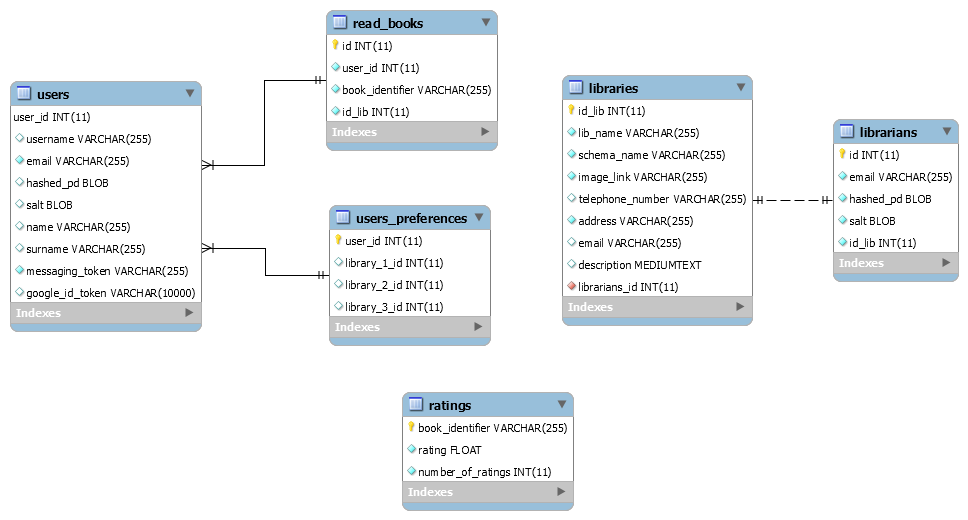
\includegraphics[scale=0.50]{Images/Diagrams/proprietary_db_UML}
	\caption{Proprietary database}
\end{figure}

\vspace*{0cm}
\begin{figure}[H]
	\centering
	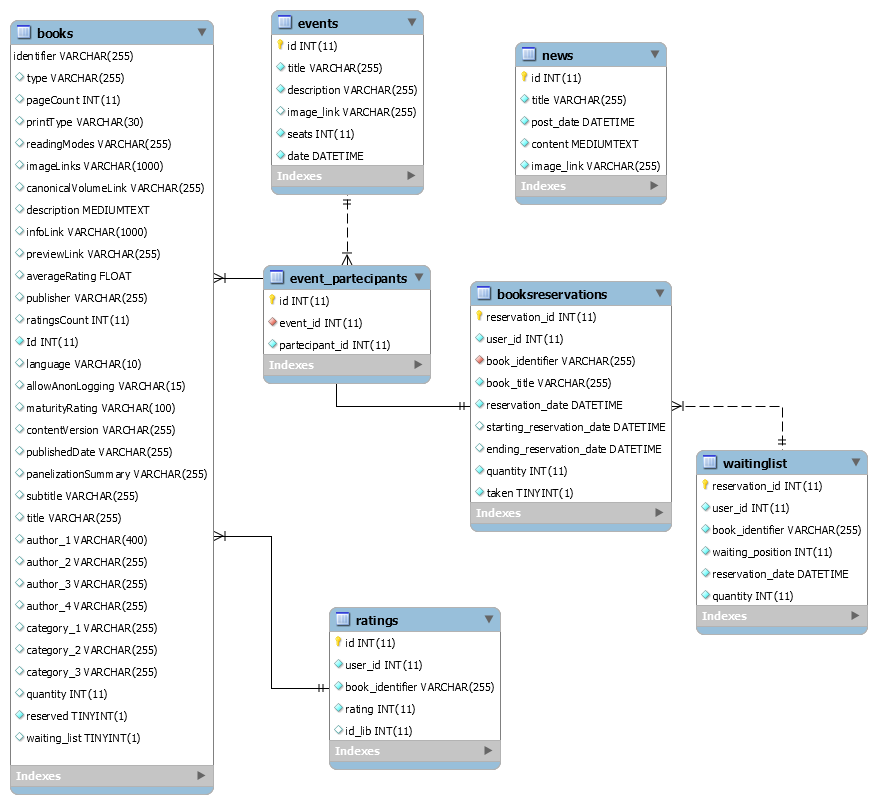
\includegraphics[scale=0.50]{Images/Diagrams/library_db_UML}
	\caption{Library database}
\end{figure}

In order to maintain the data consistency after that users perform state changing operations, we have implemented 9 triggers distributed between the various schemas and tables. We list all of them below along with the description of their behaviour.

\newpage
\mysubsubsection{Triggers - Library schema}

\begin{tabular}[H]{p{4cm}|p{4cm}|p{4cm}}
	\textbf{Trigger name} & \textbf{Table name} & \textbf{When} \\
	\hline
	\rule{0pt}{4ex} On\_insert\_rating  & ratings & after insert \\
	\hline
\end{tabular}
\vspace{0.8cm}
\\
It computes the updated average rating of a book including the inserted rating and store it in the table ratings of the proprietary\_db if it does not exist or update a currently existing record.

\vspace{0.8cm}
\begin{tabular}[H]{p{4cm}|p{4cm}|p{4cm}}
	\textbf{Trigger name} & \textbf{Table name} & \textbf{When} \\
	\hline
	\rule{0pt}{4ex} update\_count\_on
	\_delivering  & booksreservations & after delete \\
	\hline
\end{tabular}
 \vspace{0.8cm}\\
It updates the count of available copies for a book in books table in library\_x schema after that one of them has been delivered. If the current available number of copy result to be zero after the action, the Boolean reserved is set to true.


\vspace{0.8cm}
\begin{tabular}[H]{p{4cm}|p{4cm}|p{4cm}}
	\textbf{Trigger name} & \textbf{Table name} & \textbf{When} \\
	\hline
	\rule{0pt}{4ex} waiting\_list\_flowing  & booksreservations & after delete \\
	\hline
\end{tabular}
 \vspace{0.8cm}\\
It updates the position of the users in line of the book with the identifier equal to that one of the record deleted in the booksreservations table and remove the first waiting user for the book since it has to be inserted in the bookreservations table.

\vspace{0.8cm}
\begin{tabular}[H]{p{4cm}|p{4cm}|p{4cm}}
	\textbf{Trigger name} & \textbf{Table name} & \textbf{When} \\
	\hline
	\rule{0pt}{4ex} update\_on\_reservation  & booksreservations & after insert \\
	\hline
\end{tabular}
\vspace{0.8cm}
\\

It updates the count of available copies for a book in books table in library\_x schema after that one of them has been returned to the librarian of library x.

\vspace{0.8cm}
\begin{tabular}[H]{p{4cm}|p{4cm}|p{4cm}}
	\textbf{Trigger name} & \textbf{Table name} & \textbf{When} \\
	\hline
	\rule{0pt}{4ex} update\_on\_reservation  & booksreservations & after insert \\
	\hline
\end{tabular}
\vspace{0.8cm}
\\
It updates the count of available copies for a book in books table in library\_x schema after that one of them has been returned to the librarian of library x.

\vspace{0.8cm}
\begin{tabular}[H]{p{4cm}|p{4cm}|p{4cm}}
	\textbf{Trigger name} & \textbf{Table name} & \textbf{When} \\
	\hline
	\rule{0pt}{4ex} update\_available\_
	seats\_ins  & event\_partecipants & after insert \\
	\hline
\end{tabular}
\vspace{0.8cm}
\\
It updates the count of available seats for an event after a registration for it has been performed.

\vspace{0.8cm}
\begin{tabular}[H]{p{4cm}|p{4cm}|p{4cm}}
	\textbf{Trigger name} & \textbf{Table name} & \textbf{When} \\
	\hline
	\rule{0pt}{4ex} update\_available\_
	seats\_del  & event\_partecipants & after delete \\
	\hline
\end{tabular}
\vspace{0.8cm}
\\
It updates the count of available seats for an event after that a registration for it has been removed.

\vspace{0.8cm}
\begin{tabular}[H]{p{4cm}|p{4cm}|p{4cm}}
	\textbf{Trigger name} & \textbf{Table name} & \textbf{When} \\
	\hline
	\rule{0pt}{4ex} on\_insert\_waiting\_
	person  & waitinglist & before insert \\
	\hline
\end{tabular}
\vspace{0.8cm}
\\
It sets the position in the waiting list of the new user inserted in the table for a book.

\vspace{0.8cm}
\begin{tabular}[H]{p{4cm}|p{4cm}|p{4cm}}
	\textbf{Trigger name} & \textbf{Table name} & \textbf{When} \\
	\hline
	\rule{0pt}{4ex} update\_waitinglist\_
	position  & waitinglist & after delete \\
	\hline
\end{tabular}
\vspace{0.8cm}
\\
It updates the position of the users in line for a book after that a user in line has deleted is presence in the queue.

\mysubsubsection{Triggers - Proprietary schema}
\begin{tabular}[H]{p{4cm}|p{4cm}|p{4cm}}
	\textbf{Trigger name} & \textbf{Table name} & \textbf{When} \\
	\hline
	\rule{0pt}{4ex} on\_insert\_rating
	\_propDB  & ratings & after insert \\
	\hline
\end{tabular}
\vspace{0.4cm}
\\
It updates the average rating for the considered book in all the libraries of the system.
\vspace{0.4cm}



\mysubsubsection{Internal customized data structures}
In order to make the communication easier and the data transmission between the clients and the application server manageable, we have created few serializable data structures that are sent over the internet. They are 13 java classes designed with the purpose of containing all the information that server and clients need to exchange such as: books information, reservation details, events schedule, etc. 

\mysubsection{Deployment View}
Here we provide a deployment strategy for our system.

\vspace*{0cm}
\begin{figure}[H]
	\centering
	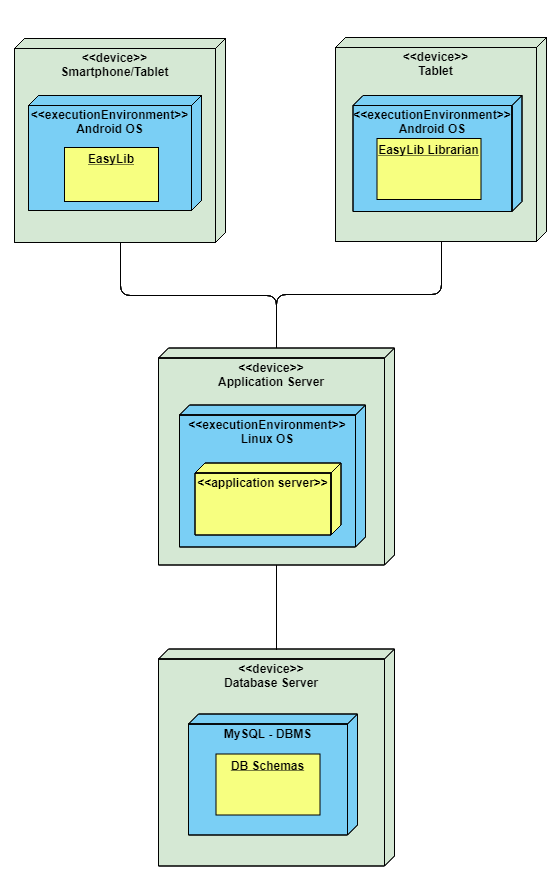
\includegraphics[scale=0.55]{Images/Diagrams/Deployment_view_EasyLib}
	\caption{Deployment view EasyLib}
\end{figure}

\newpage
\mysubsection{Non-Functional Requirements}
Here we state some non functional requirements that our system must respect during the execution.

\begin{itemize}
\item \emph{Performance:} The system must be able to respond to a consistent number of user requests simultaneously. All the data requested by the users and the needed computations must respectively retrieved and performed as soon as possible and as efficiently as possible.

\item \emph{Reliability:} The system must guarantee a 24/7 service. The information must be stored in proprietary Database in order to be always available to the user when required.
\item \emph{Scalability:} The system must ensure a high level of scalability, since new libraries can join the system in any moment enlarging EasyLib supply.
\item \emph{Security:} All users’ passwords are encrypted using a hash function with salt. In this way the attacker cannot see the plain text password and steal sensitive information.

\item \emph{Accuracy:} The data retrieved by the application has to be accurate and up-to-date in a real-time fashion.
\end{itemize}